\chapter{Simulation}

\section{The many-body wavefunction}
In electronic structure calculations we are ultimately interested in the many-body wavefunction

\[ \Psi(\bm{r}_1,\bm{r}_2,\dots, \bm{r}_n; \bm{R}_1, \bm{R}_2, \dots , \bm{R}_N) \]

\noindent where $\bm{r}_i$ are electron coordinates and $\bm{R}_i$ are nuclear coordinates. Imagine that we want to calculate this object for a small molecule such as Benzene (C$_6$H$_6$) containing 12 nuclei and 42 electrons. This wavefunction exists in $42\cdot3-6 = 156$ dimensional cartesian space! If we want to store this object on a computer with a modest precision of 10 grid points per coordinate, it would require $10^{156}$ complex numbers or $64 \cdot 10^{156}$ bits (assuming single-precision floating points numbers of 32 bits). Lloyd2000 estimated the total number of bits available for computation in the observable universe to be $10^{90}$ (Lloyd2000). Even with the entire universe at our disposal this object is completely unmanageable. This exercise also emphasizes the potential of Quantum Computers. For this reason, we fix the ionic positions and assume that the many-body wavefunction can be written as a product of single-electron wavefunctions (orbitals):

\[ \Psi(\bm{r}_1,\bm{r}_2,\dots, \bm{r}_n; \bm{R}_1, \bm{R}_2, \dots , \bm{R}_N) \longrightarrow \phi(\bm{r}_1)\phi(\bm{r}_2)\dots\phi(\bm{r}_n) \]

\section{Band paths}

\begin{figure}
    \centering
    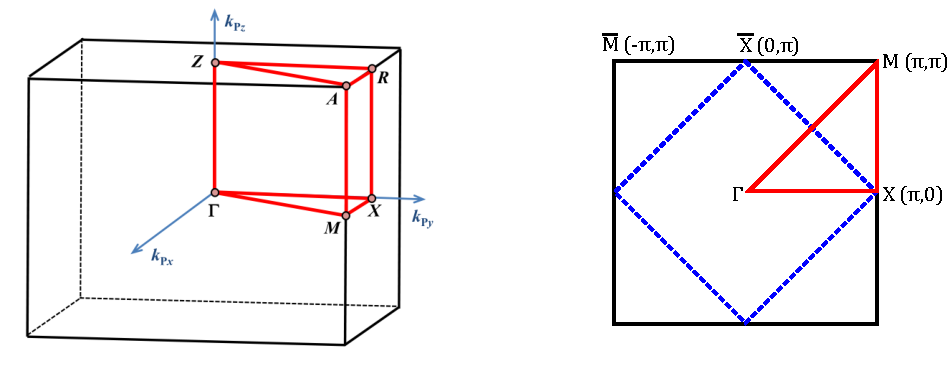
\includegraphics{fig/simulation/band_paths.pdf}
    \caption[Band paths]{\textbf{Left:} BZ of a primitive tetragonal cell with high-symmetry lines. \textbf{Right:} The in-plane BZ with the same labels and the usual $\Gamma$-$X$-$M$-$\Gamma$ path. If the large BZ is the crystallographic HTT phase, then the broken blue lines represent the LTO/LTT/LTLO BZ and we can consider the $\Gamma$-$X$-$\frac{M}{2}$-$\Gamma$ path, since $M$ becomes $\Gamma$ for this (smaller) BZ. In literature the labels are often confused, while $(\pi,\pi)$ and $(\pi,0)$ are universally agreed upon. In any band structure diagrams presented here, the labels in this figure is used.} 
    \label{fig:band_paths}
\end{figure}

\begin{figure}
    \centering
    \[
    \text{PA(HTT)} =  
    \begin{pmatrix}
    0 & 0 & \frac{1}{2} \\
    \frac{1}{2} & \bar{\frac{1}{2}} & 0 \\
    \frac{1}{2} & \frac{1}{2} & \bar{\frac{1}{2}}
    \end{pmatrix}
    \qquad
    \text{PA(LTO)} =  
    \begin{pmatrix}
    \frac{1}{2} & \frac{1}{2} & 0 \\
    0 & 0 & 1 \\
    \frac{1}{2} & \bar{\frac{1}{2}} & 0
    \end{pmatrix}
\]
    \caption[Transformation matrices]{Transformation matrix from the orthorhombic crystallographic unit cell (Bmab) to primitive cells in the HTT/LTO phases. For LTT and LTLO the transformation matrix is the identity. Since band structure calculations (bands/electronic) are based on primtive cells, these matrices can be used to generate $k$-points starting from the more `intuitive' notation outlined in Figure \ref{fig:band_paths}. For example, the $X$-point ($(\frac{1}{2} \frac{1}{2} 0)$ wrt LTT) in the HTT phase becomes $(\frac{1}{2} \frac{1}{2} 0) \cdot \text{PA(HTT)} = (\frac{1}{4} \bar{\frac{1}{4}} \frac{1}{4})$}
    \label{fig:primtive_axes}
\end{figure}

\section{Octahedral tilts}
We are interested in describing the distances $d_y$ and $d_z$ as a function of the tilt angle as shown in Figure \ref{fig:tilt}(right). Our coordinate system is usually given in terms of lattice constants that define the coordinate system and scaled coordinates. To do the rigid rotation, we thus need to perform some transformations in order to make sure the tilt angles are with reference to the real-space lattice.

\begin{figure}
    \centering
    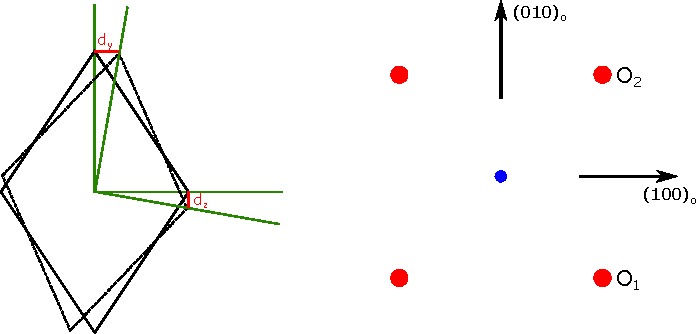
\includegraphics[width=0.8\textwidth]{fig/simulation/tilt.pdf}
    \caption[Geometry of octahedral tilts]{Left: Geometry of octahedral tilts in the with the $c$-axis vertical. Right: Illustration of the two inequivalent in-plane oxygens. The $Q_1$ irreducible representation represents a rotation around the (010) axis while $Q_2$ is a rotation around the (100) axis.}
    \label{fig:tilt}
\end{figure}

All possible tilts can be described with reference to the LTLO (Pccn) phase. The octahedra are described with two in-plane oxygens (O$_1$, O$_2$) and one apical oxygen $O_3$. Due to symmetry constrains, a rotation of this octahedron will cause a displacements in the $z$-direction of the in-plane oxygen and in the $a$- and $b$-directions of the apical oxygen. Following \cite{Axe1989}, we define $Q_1$ as a rotation around the (010) axis and $Q_2$ as a rotation around the (100) axis in orthorhombic notation. In more intuitive terms, $Q_1$ `tilts' the octahedron along $x$, while $Q_2$ `tilts' along $y$.

By inspection of Figure \ref{fig:tilt}, a $Q_1$ rotation will displace O$_3$ in the $x$-direction and O$_1$, O$_2$ in the negative $z$-direction. A $Q_2$ rotation will displace O$_3$ in the $y$-direction, O$_1$ in the positive $z$-direction and O$_2$ in the negative $z$-direction. If we want to express $Q_1$ and $Q_2$ as angles, the displacements become:


\begin{align*}
d_x(\text{O}_3) &= | \text{O}_\text{ap} | \sin (Q_1) \frac{c}{a} \\
d_y(\text{O}_3) &= | \text{O}_\text{ap} | \sin (Q_2) \frac{c}{b} \\
d_z(\text{O}_1) &= \frac{1}{4c} \left[ - a \sin (Q_1) + b \sin (Q_2) \right] \\
d_z(\text{O}_2) &= \frac{1}{4c} \left[ - a \sin (Q_1) - b \sin (Q_2) \right] \, ,
\end{align*}

\noindent where $| \text{O}_\text{ap} |$ is the apical oxygen distance, or the $z$-component of O$_3$. Since these equations uniquely define displacements in terms of tilt angles, we can also find tilt angles from structural displacements from either the apical oxygen:

\begin{align*}
Q_1 &= \sin^{-1} \left( \frac{d_x(\text{O}_3)}{| \text{O}_\text{ap} |} \times \frac{a}{c} \right) \\
Q_2 &= \sin^{-1} \left( \frac{d_y(\text{O}_3)}{| \text{O}_\text{ap} |} \times \frac{b}{c} \right) \, ,
\end{align*}

\noindent or the equatorial oxygen:

\begin{align*}
Q_1 &= \sin^{-1}  \left( - \frac{2c}{a} \times (d_z(\text{O}_1) + d_z(\text{O}_2)) \right) \\
Q_2 &= \sin^{-1}  \left( -\frac{4c}{b} \times d_z(\text{O}_2) - \frac{a}{b} \times \sin (Q_1) \right) \, .
\end{align*}

These equations can then be used to generate desired tilts and extract tilt angles from a structural minimization.

\section{Equation of state fits}

Equation of state fit based on Vinet's exponential equation of state \cite{Vinet1987}:

\begin{equation*}
\tiny
E(V) = E_0 + \frac{2B_0V_0}{\left(B_0^\prime-1\right)^2}\left\lbrace 2 -\left[ 5 + 3\left( \frac{V}{V_0}\right)^\frac{1}{3} (B_0^\prime -1)  -3B_0^\prime \right] \right. \left. \exp \left[ -\frac{3}{2} \left( B_0^\prime-1\right)\left[\left( \frac{V}{V_0}\right)^\frac{1}{3} -1\right]\right]\right\rbrace
\end{equation*}

\noindent where $V_0$ is the equilibrium volume, $B_0$ is the equilibrium bulk modulus and 

\begin{equation*}
    B_0^\prime = \left( \frac{\partial B_0}{\partial P}\right)_T
\end{equation*}

\section{MD}
Temperature fluctuations in a closed system:

\[ \frac{\Delta T}{T} = \sqrt{\frac{2}{3N}} \quad \Rightarrow \quad \Delta T(T=\SI{300}{\kelvin}) = \SI{23.1}{\kelvin} \]

\noindent Nose-Hover algorithm:

\begin{align*}
v_i^\text{scaled} &= \frac{\bm{p}_i}{m_i} \\
\text{d}\bm{p}_i &= (\bm{F}_i - \zeta \bm{p}_i) \text{d}t \\
\text{d}\zeta &= \frac{1}{Q} \left( \sum_{i=1}^N \frac{|\bm{p_i}|^2}{m_i} - (3N+1)k_\text{B}T\right) \text{d}t
\end{align*}

\begin{table}[b]
\centering
\begin{tabular}{@{}lll@{}}
\toprule
 & Core (\# electrons) & Valence (\# electrons)                        \\ \midrule
\texttt{La}                 & Kr4d$^{10}$ (46)                & 5s$^1$6s$^2$5p$^6$5d$^1$ (11) \\
\texttt{Cu\_pv}                 & 1s$^2$2s$^2$2p$^6$3s$^2$ (12) & 3p$^6$3d$^{10}$4s$^1$ (17)      \\
\texttt{O}                  & 1s$^2$ (2)                    & 2s$^2$2p$^4$ (6)              \\ \bottomrule
\end{tabular}
\caption[VASP Pseudopotentials]{Psedopotenial electronic configuration used in VASP calculations.}
\label{tab:vasp_pseudo}
\end{table}

\begin{figure}
    \centering
    \begin{lstlisting}[basicstyle=\footnotesize\ttfamily, frame=single]
    ENCUT = 520 # 1.3x suggested value from O POTCAR, 800 for phonons
    EDIFF = 1E-5 # 1E-8 for phonons
    ALGO = NORMAL
    PREC = Accurate
    ADDGRID = .FALSE.
    LREAL = Auto # Switch to .FALSE. for phonons
    
    ISPIN = 2
    MAGMOM = 1 -1 1 -1 24*0 # AFM structure
    
    ISMEAR = 0
    SIGMA = 0.1
    
    LDAU= .TRUE. # Enable LDA+U with U=8eV and J=0.8eV
    LDAUTYPE = 4 # No exchange splitting
    LDAUL = 2 -1 -1 # only on Cu d states
    LDAUU = 8 0 0 
    LDAUJ = 0.8 0 0
    \end{lstlisting}
    \caption[VASP: Typical INCAR]{Typical INCAR for VASP simulations.}
    \label{fig:incar}
\end{figure}

\begin{figure}
    \centering
    \[
    \text{I4/mmm} \quad 
    \begin{pmatrix}
    1 & \bar{1} & 0 \\
    1 & 1 & 0 \\
    0 & 0 & 1
    \end{pmatrix}
    \quad \text{Bmab}
\]

\[
    \text{I4/mmm} \quad 
    \begin{pmatrix}
    1 & 1 & 0 \\
    1 & \bar{1} & 0 \\
    1 & 0 & \bar{1}
    \end{pmatrix}
    \quad \text{Bmab} \quad
    \begin{pmatrix}
    1 & 0 & 1 \\
    0 & 1 & 0 \\
    \bar{1} & 0 & 1
    \end{pmatrix} 
    \quad \text{P4}_2\text{/ncm}
\]
    \caption[Structural transformation matrices]{Structural transformation matrices between HTT (I4/mmm), LTO (Bmab) and LTT (P4$_2$/ncm). Top: Conventional cells. Bottom: Primitive cells. LTT and LTO conventional are identical. NB: In \texttt{CRYSTAL17} the expansion matrices are transposed with respect to the ones shown in the figure. In e.g. \texttt{VESTA} they can be used directly. This distinction only matters for the I4/mmm to Bmab primitive transformation (which is needed to describe anti-ferromagnetism in LTT). For the others it just changes the direction of rotation.}
    \label{fig:matrices}
\end{figure}

\begin{figure}
    \centering
    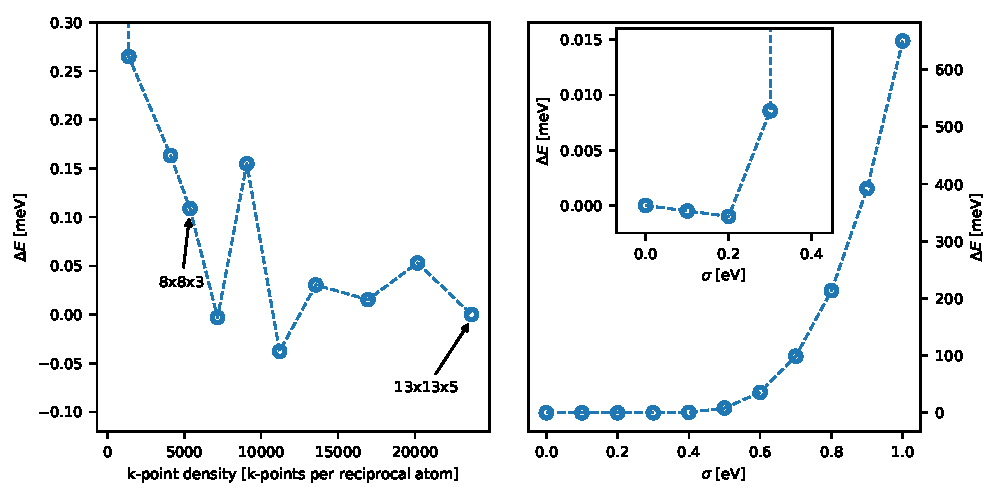
\includegraphics{fig/simulation/convergence_afm.pdf}
    \caption[Simulation Benchmarks: GGA+U]{Simulation Benchmarks: GGA+U with $U=\SI{8}{\eV}$ and $J=\SI{0.8}{\eV}$. \textbf{Left:} Energy as a function of k-point density with $\sigma=\SI{0.1}{\eV}$. $\Delta E$ is total energy (with entropy) with respect to the $13 \times 13 \times 5$ mesh. \textbf{Right:} $\Delta E$ as a function of smearing $\sigma$, where $\sigma=0$ corresponds to the tetrahedron method (\texttt{ISMEAR=-5}).}
    \label{fig:sim_bench_afm}
\end{figure}

\begin{figure}
    \centering
    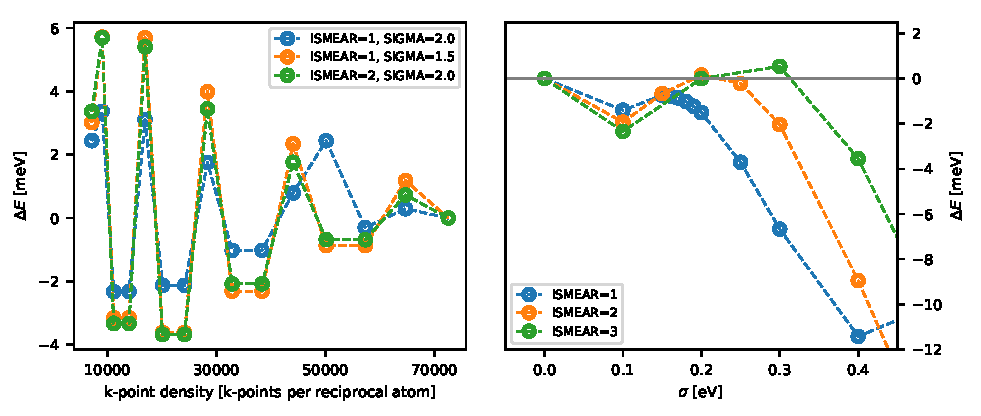
\includegraphics{fig/simulation/convergence_metal.pdf}
    \caption[Simulation Benchmarks: Paramagnet/Metal]{Simulation Benchmarks: Paramagnet/Metal. Note the significant variation in energy compared to the insulating case, even with much higher k-point density. \textbf{Left:} Energy as a function of k-point density for three combinations values of $\sigma$ and smearing type. $\Delta E$ is total energy (with entropy) with respect to the $18 \times 18 \times 8$ mesh. \textbf{Right:} $\Delta E$ as a function of $\sigma$ with the Methfessel-Paxton method (orders 1, 2, 3) while using a $16 \times 16 \times 8$ k-point mesh (57344 k-points per reciprocal atom). $\sigma=0$ corresponds to the tetrahedron method (\texttt{ISMEAR=-5}). Below $\sigma = \SI{0.4}{\eV}$ the entropy term is \SI{0.5}{\milli\eV} per atom or lower, so forces should be well-behaved.}
    \label{fig:sim_bench_para}
\end{figure}

\begin{table}[b]
    \centering
    \begin{tabular}{@{}llll@{}}
    \toprule
    U [eV] & J [eV] & Moment [$\mu_\text{B}$] & Optical gap [eV] \\ \midrule
    4.0    & 0.4    & 0.330       & 0.348    \\
    6.0    & 0.6    & 0.481       & 1.016    \\
    8.0    & 0.8    & 0.588       & 1.686    \\
    10.0   & 1.0    & 0.676       & 1.877    \\
    12.0   & 1.2    & 0.755       & 2.042    \\ \bottomrule
    \end{tabular}
    \caption[LDA+U Benchmarking]{LDA+U Benchmarking}
    \label{tab:ldau}
\end{table}

\begin{table}[b]
    \centering
    \begin{tabular}{@{}lllll@{}}
    \toprule
               & HTT & HTT (metal)  & LTO    & LTT    \\ \midrule
    a [\AA]         & 5.32 & 5.31 & 5.34   & 5.37   \\
    c [\AA]         & 12.99 & 13.05 & 13.01  & 12.93  \\
    O3(z)      & 0.184 & 0.185 & 0.185  & 0.184  \\
    La(x)      & 0     & 0 & 0      & -0.009 \\
    La(y)      & 0     & 0 & -0.012 & -0.009 \\
    La(z)      & 0.362 & 0.362 & 0.361  & 0.361  \\
    $\eta$ ($\times 100$) & 0  & 0 &  1.465  & 0      \\
    Q1 (degrees)        & 0 & 0 &  0      & 4.6125 \\
    Q2 (degrees)        & 0 & 0 &  5.786  & 4.6125 \\ 
    degrees of freedom & 2 & 2 & 5 & 5 \\ \bottomrule
    \end{tabular}
    \caption[HTT, LTO, LTT: Structural parameters]{HTT, LTO, LTT: Structural parameters, defined with a minimal set of parameters based on results from simulations. Q1/Q2 are taken as the average angle from equatorial and apical tilt. The fractional positions of O1, O2 and O3 are completely described using Q1, Q2 and O3(z), Cu is allways at (0,0,0) and $\eta = \frac{b-a}{b+a}$ uniquely defines any difference between $a$ and $b$. In the generation of structures, the Pccn (LTLO) space group is used. Degrees of freedom refers to the atomic positions only. The description of our system in terms of Q1/Q2 thus removes one degree of freedom by coupling the apical and equatorial oxygen.}
    \label{tab:struct_par}
\end{table}



\begin{figure}
    \centering
    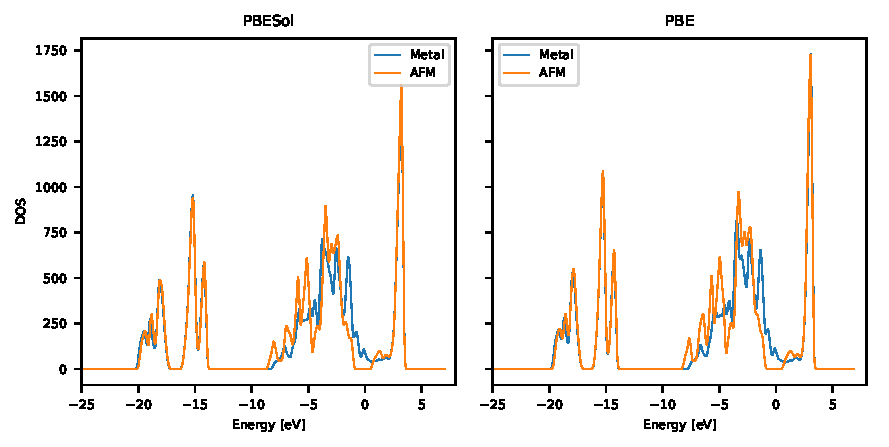
\includegraphics{fig/simulation/htt_dos.pdf}
    \caption[Electronic DOS: Metal and AFM]{Electronic density of states for HTT phase with two different functionals in a metallic (paramagnetic) and AFM (GGA+U) states. The two functionals appear to describe the system identically. The AFM state is shifted by \SI{-1}{\eV} for comparative purposes (which is why the Fermi level is in the middle of the gap).}
    \label{fig:edos_htt}
\end{figure}

\begin{figure}
    \centering
    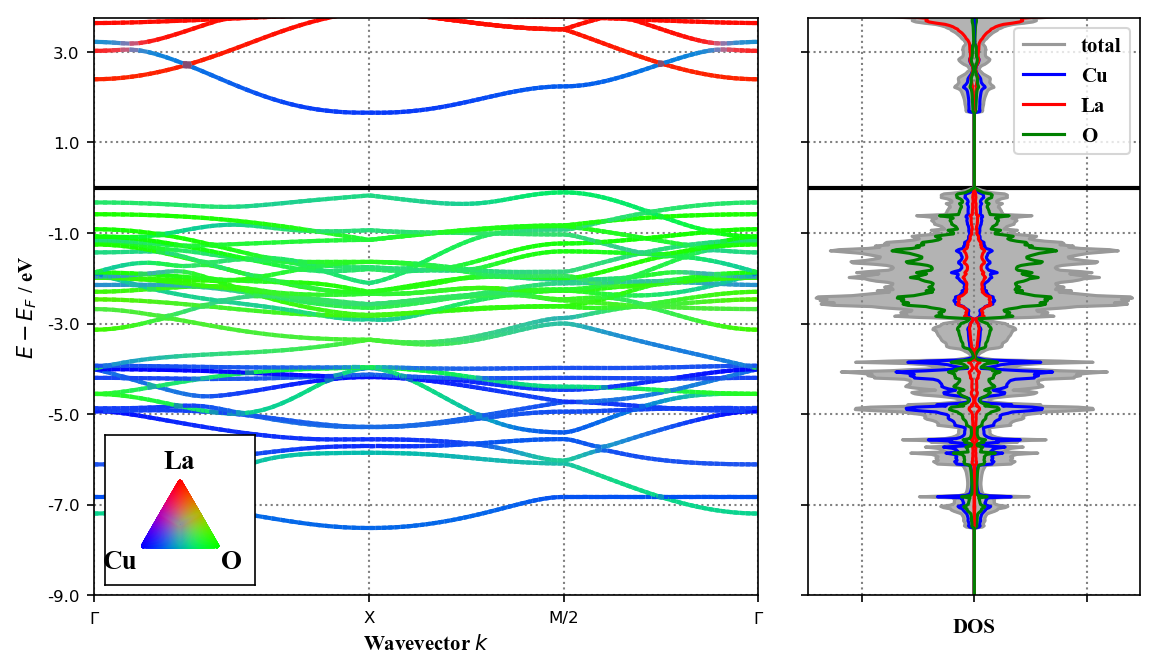
\includegraphics[width=\textwidth]{fig/simulation/bs_afm2.png}
    \caption[GGA+U: AFM Electronic Band Structure]{GGA+U: AFM Electronic Band Structure of the Bmab LTO structure along the $\Gamma$-$X$-$\frac{M}{2}$-$\Gamma$ path (LTO high symmetry lines). The upper and lower Hubbard bands are clearly visible and are separated by \SI{8}{\eV} as expected.}
    \label{fig:bs_afm2}
\end{figure}

\begin{figure}
    \centering
    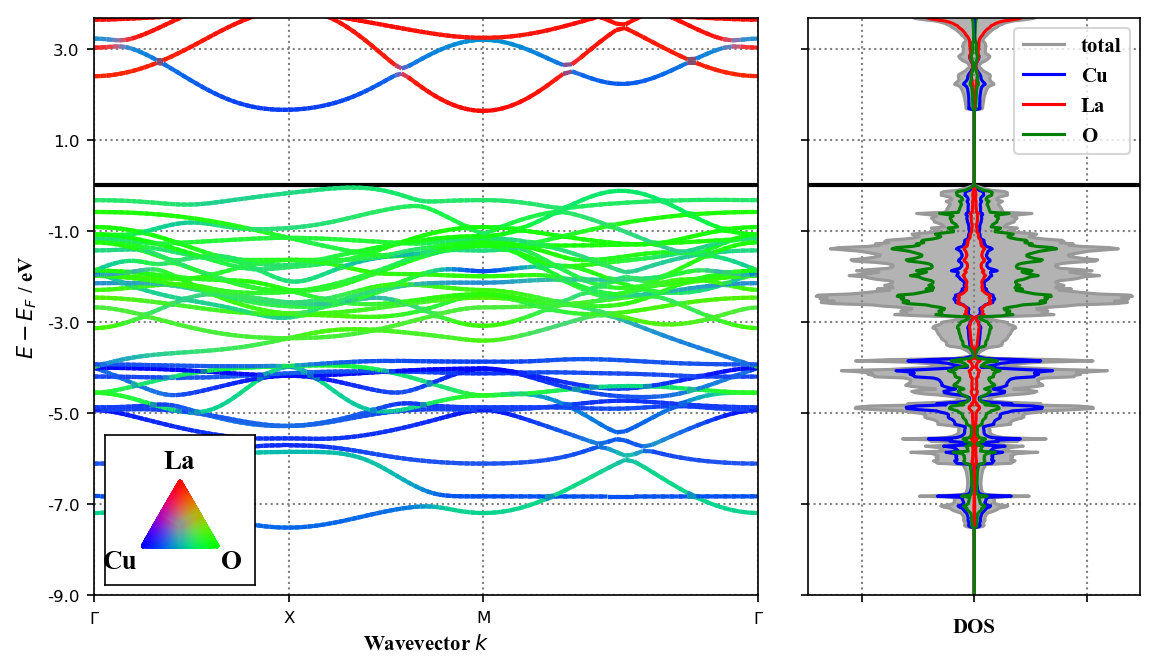
\includegraphics[width=\textwidth]{fig/simulation/bs_afm1.png}
    \caption[GGA+U: AFM Electronic Band Structure]{GGA+U: AFM Electronic Band Structure of the Bmab LTO structure along the $\Gamma$-$X$-$M$-$\Gamma$ path (HTT high symmetry lines). The upper and lower Hubbard bands are clearly visible and are separated by \SI{8}{\eV} as expected.}
    \label{fig:bs_afm1}
\end{figure}

\begin{figure}
    \centering
    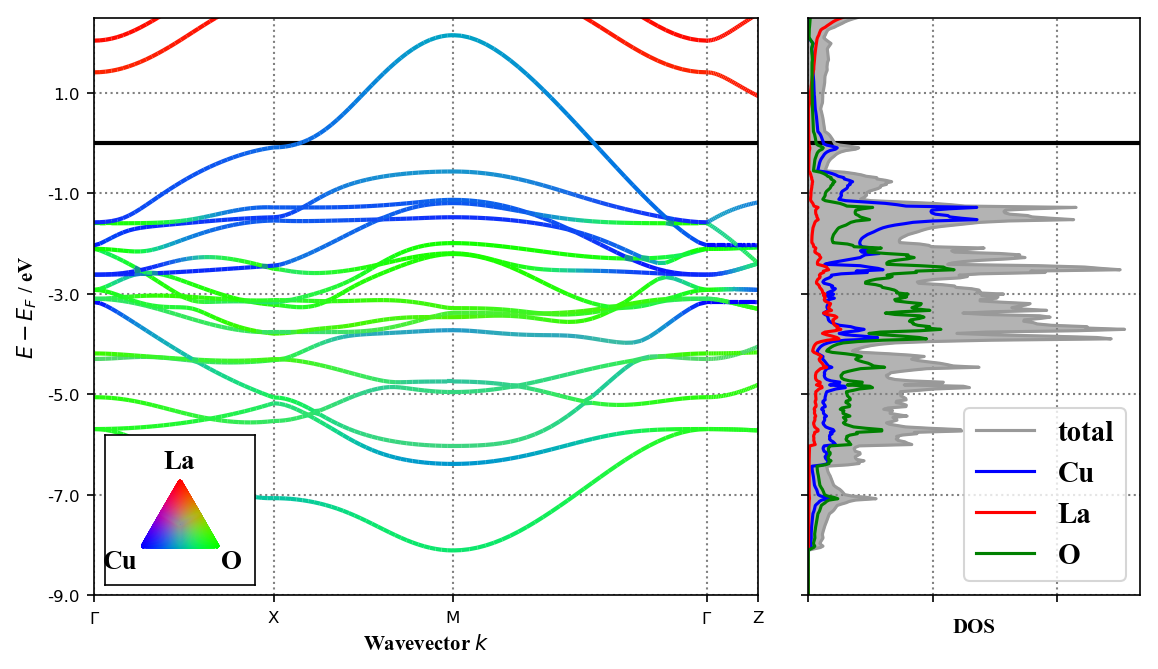
\includegraphics[width=\textwidth]{fig/simulation/bs_metal.png}
    \caption[GGA: Metallic Electronic Band Structure]{Metallic Electronic Band Structure of the I4/mmm HTT structure. Path is through the high-symmetry points as defined in Figure \ref{fig:band_paths} with respect to the conventional unit cell. The $\Gamma$-$Z$ path is shown to illustrate the 2-dimensional nature of the electronic structure (The dispersion is relatively flat).}
    \label{fig:bs_metal}
\end{figure}

\begin{figure}
    \centering
    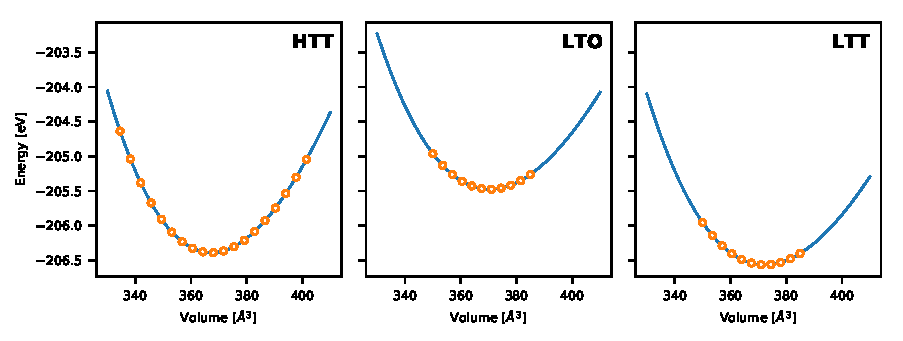
\includegraphics[width=\textwidth]{fig/simulation/eos_all.pdf}
    \caption[AFM: Equation-of-state fits]{Equation-of-state fits (AFM). Optimal volume of simulated structures are found by performing optimization of fractional coordinates and cell shape at a series of fixed volumes. The resulting Energy/Volume curve is then fit to a Vinet exponential equation of state \cite{Vinet1987}. This is done for the HTT, LTO and LTT phases with the PBESol functional.}
    \label{fig:eos_all}
\end{figure}

\begin{figure}
    \centering
    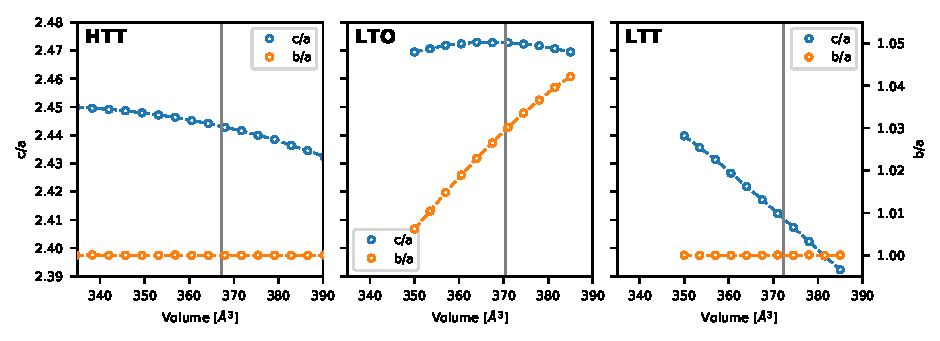
\includegraphics[width=\textwidth]{fig/simulation/ratio_all.pdf}
    \caption[AFM: Cell ratios during EOS fits]{Cell Ratios (AFM). During the equation-of-states fits from Figure \ref{fig:eos_all}, the cell shape is modified, changing the $b/a$ ratio (orthorhombicity) and $c/a$ ratio (larger values correspond to a cell that is elongated along $c$). Due to symmeetry $b/a = 1$ for the HTT and LTT phases. Vertical line is the optimal volume from the fit.}
    \label{fig:eos_ratios}
\end{figure}

\begin{figure}
    \centering
    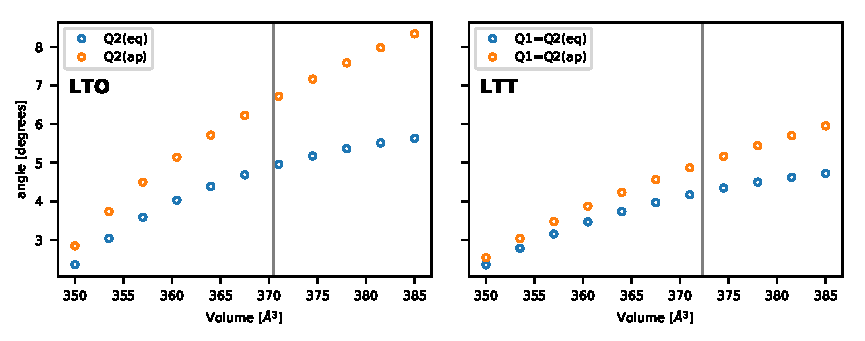
\includegraphics[width=\textwidth]{fig/simulation/angles_lto_ltt.pdf}
    \caption[AFM: LTO/LTT angles during EOS fits]{LTO/LTT Angles (AFM) During equation-of-state fits (Figure \ref{fig:eos_all}, we record the tilt angles for the LTO and LTT phase. Here, they are plotted as a function of Volume. Note that for LTO $Q_1=0$ and for LTT $Q_1=Q_2$. However, the rotation angle is measured differently from the equatorial (eq) and apical (ap) oxygen. The difference in values can be thought of as `non-rigidity' of the rotation.}
    \label{fig:my_label}
\end{figure}


\begin{figure}
    \centering
    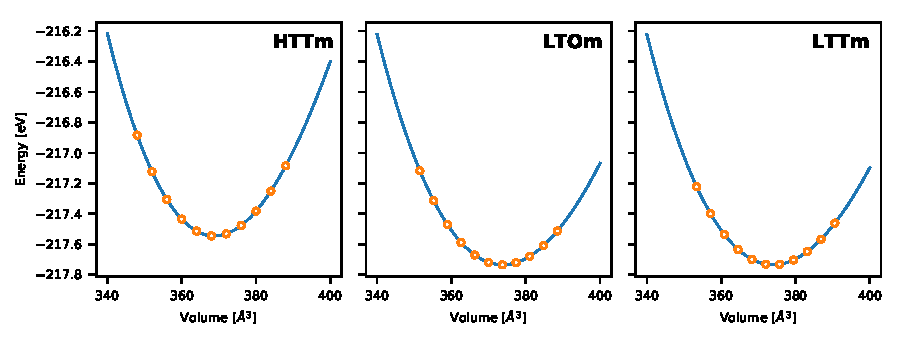
\includegraphics[width=\textwidth]{fig/simulation/eos_metal_all.pdf}
    \caption[Metal: Equation-of-state fits]{Equation-of-state fits (Metal). Optimal volume of simulated metallic structures are found by performing optimization of fractional coordinates and cell shape at a series of fixed volumes. The resulting Energy/Volume curve is then fit to a Vinet exponential equation of state \cite{Vinet1987}. This is done for the HTT, LTO and LTT phases with the PBESol functional.}
    \label{fig:eos_metal_all}
\end{figure}

\begin{figure}
    \centering
    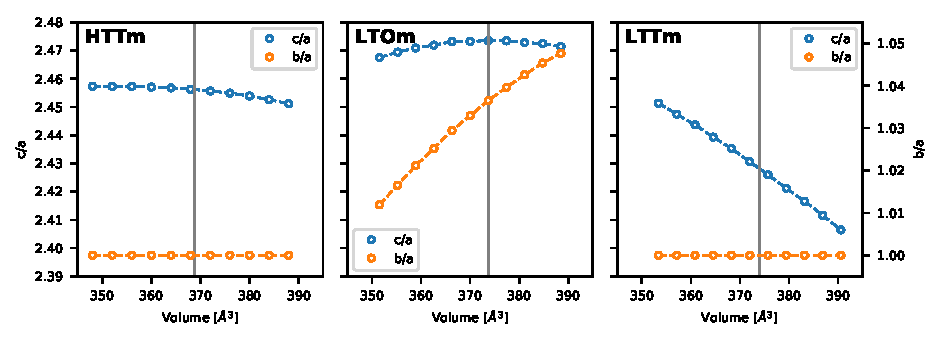
\includegraphics[width=\textwidth]{fig/simulation/ratio_metal_all.pdf}
    \caption[Metal: Cell ratios during EOS fits]{Cell ratios (Metal). During the equation-of-states fits from Figure \ref{fig:eos_metal_all}, the cell shape is modified, changing the $b/a$ ratio (orthorhombicity) and $c/a$ ratio (larger values correspond to a cell that is elongated along $c$). Due to symmeetry $b/a = 1$ for the HTT and LTT phases. Vertical line is the optimal volume from the fit.}
    \label{fig:eos_ratios}
\end{figure}

\begin{figure}
    \centering
    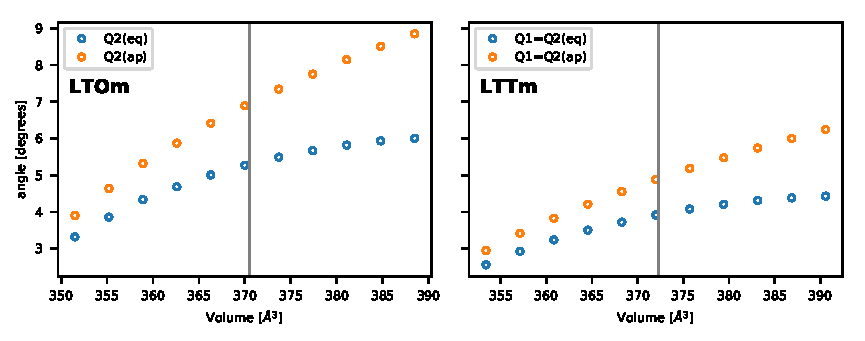
\includegraphics[width=\textwidth]{fig/simulation/angles_metal_lto_ltt.pdf}
    \caption[Metal: LTO/LTT angles during EOS fits]{LTO/LTT angles (Metal). During equation-of-state fits (Figure \ref{fig:eos_all}, we record the tilt angles for the LTO and LTT phase. Here, they are plotted as a function of Volume. Note that for LTO $Q_1=0$ and for LTT $Q_1=Q_2$. However, the rotation angle is measured differently from the equatorial (eq) and apical (ap) oxygen. The difference in values can be thought of as `non-rigidity' of the rotation.}
    \label{fig:my_label}
\end{figure}

\begin{table}[b]
    \centering
    \begin{tabular}{lllllllllll}
\toprule
structure &  phase & encut &      XC &       E0 &       V0 &    c/a &    $\eta$ &     $Q_1$ &     $Q_2$ \\
\midrule
      HTT &    afm &   520 &     PBE & -194.352 &  383.410 &  2.431 &  0.000 &  0.000 &  0.000 \\
      HTT &    afm &   800 &     PBE & -194.494 &  383.297 &  2.430 &  0.000 &  0.000 &  0.000 \\
      HTT &    afm &   800 &  PBESol & -206.390 &  367.310 &  2.443 &  0.000 &  0.000 &  0.000 \\
      LTO &    afm &   800 &  PBESol & -205.476 &  370.500 &  2.437 &  1.465 &  0.000 &  5.786 \\
      LTT &    afm &   800 &  PBESol & -206.565 &  372.282 &  2.410 &  0.000 &  4.612 &  4.612 \\
      HTT &  metal &   800 &  PBESol & -217.546 &  368.774 &  2.456 &  0.000 &  0.000 &  0.000 \\
      LTO &  metal &   800 &  PBESol & -217.735 &  373.793 &  2.430 &  1.795 &  0.000 &  6.421 \\
      LTT &  metal &   800 &  PBESol & -217.735 &  373.948 &  2.428 &  0.000 &  4.528 &  4.528 \\
\bottomrule
\end{tabular}

    \caption[Simulation Structure Results]{Resulting structure due to EOS fits to various structural phases and functionals. The two values given for $Q_1$/$Q_2$ are angles calculated from equatorial and apical oxygens, respectively. Interestingly, in terms of energy LTT $<$ HTT $<$ LTO, while the phonons are `more unstable' for HTT than LTO (See Figures \ref{fig:htt_ps}, \ref{fig:lto_ps}, \ref{fig:ltt_ps}). For the metallic cases, we note the optimal geometry is similar to the magnetic case. While the energy is lower, it is not meaningful to compare total energies between GGA+U and GGA.}
    \label{tab:sim_struct}
\end{table}

\begin{figure}
    \centering
    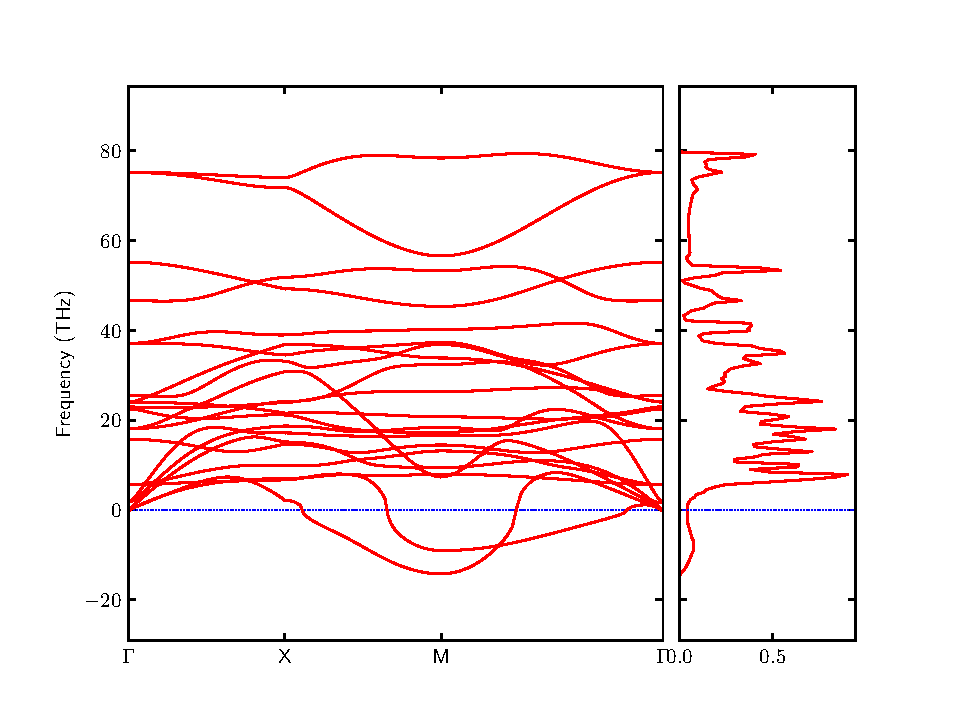
\includegraphics[width=\textwidth]{fig/simulation/band_dos_htt_pe.pdf}
    \caption[HTT Phonons (PBE)]{Phonons in HTT phase with PBE functional. Units are meV (the label is wrong). Note the problems with $\Gamma$ phonons.}
    \label{fig:htt_pe}
\end{figure}

\begin{figure}
    \centering
    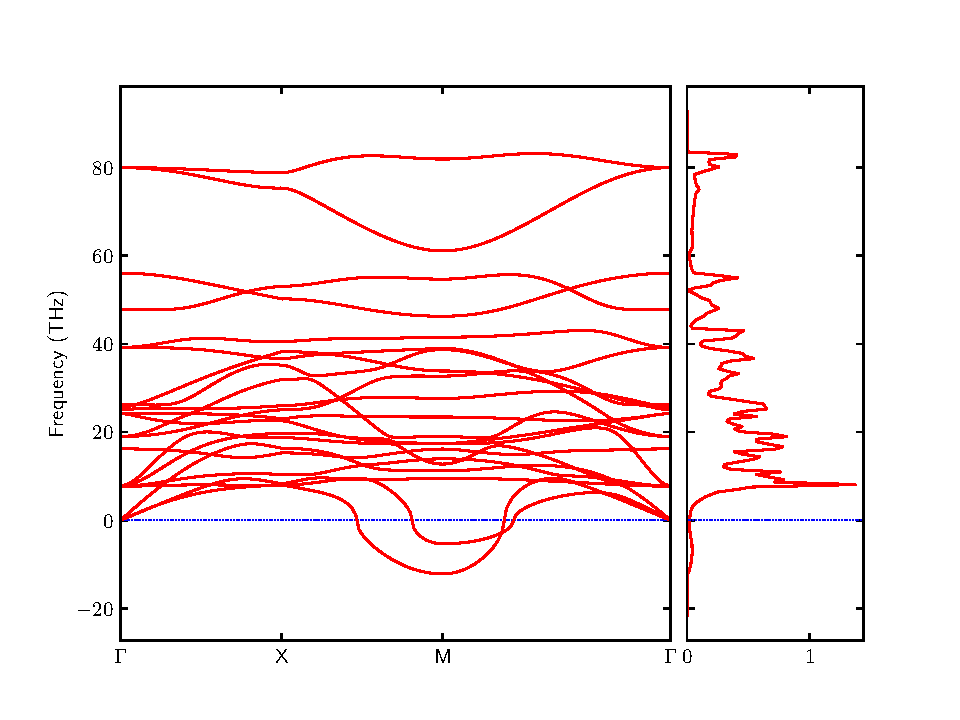
\includegraphics[width=\textwidth]{fig/simulation/band_dos_htt_ps.pdf}
    \caption[HTT Phonons (PBESol)]{Phonons in HTT phase with PBESol functional. Units are meV (the label is wrong). Note $\Gamma$ phonons are fixed.}
    \label{fig:htt_ps}
\end{figure}

\begin{figure}
    \centering
    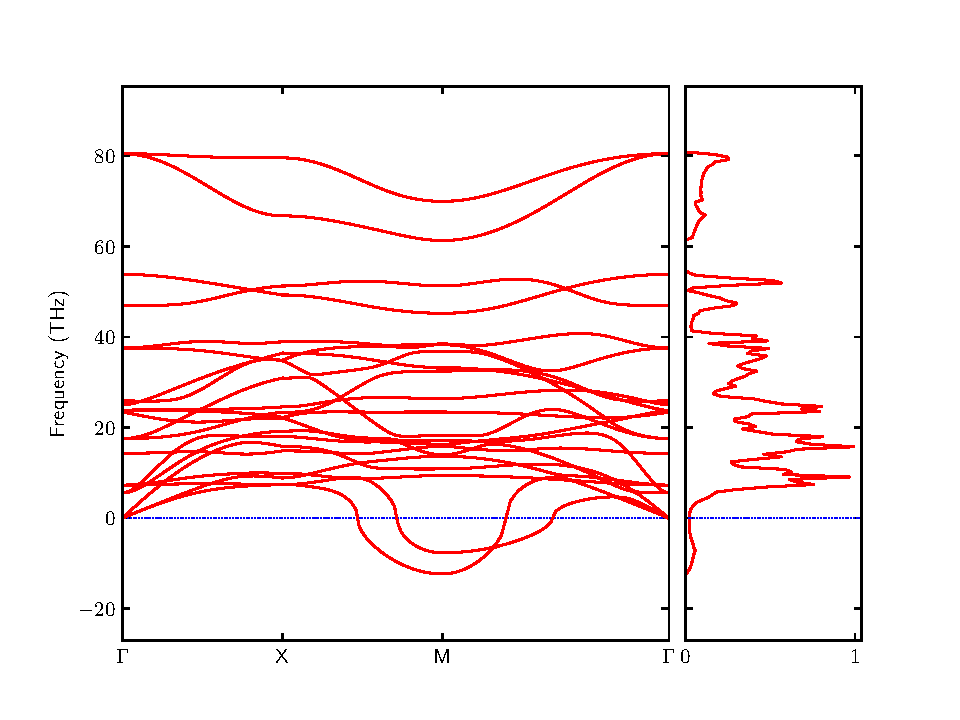
\includegraphics[width=\textwidth]{fig/simulation/band_dos_htt_metal.pdf}
    \caption[HTT Phonons (PBESol, Metal)]{Metallic Phonons in HTT phase with PBESol functional. Units are meV (the label is wrong). Note $\Gamma$ phonons are fixed.}
    \label{fig:htt_metal_ph}
\end{figure}

\begin{figure}
    \centering
    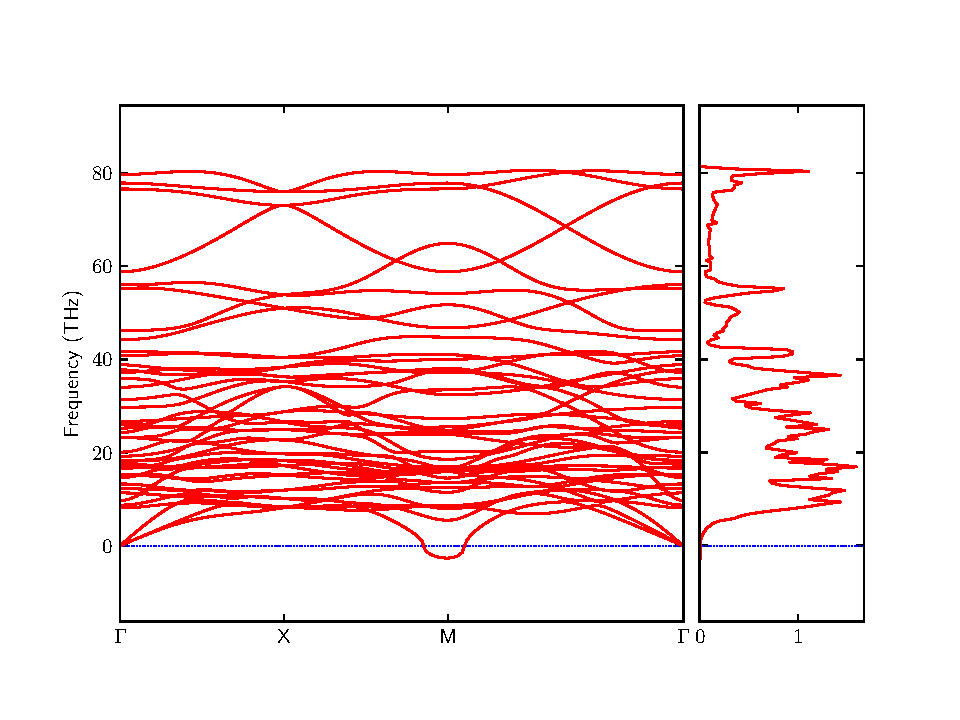
\includegraphics[width=\textwidth]{fig/simulation/band_dos_lto.pdf}
    \caption[LTO Phonons (PBESol)]{Phonons in LTO phase with PBESol functional. Units are meV (the label is wrong).}
    \label{fig:lto_ps}
\end{figure}

\begin{figure}
    \centering
    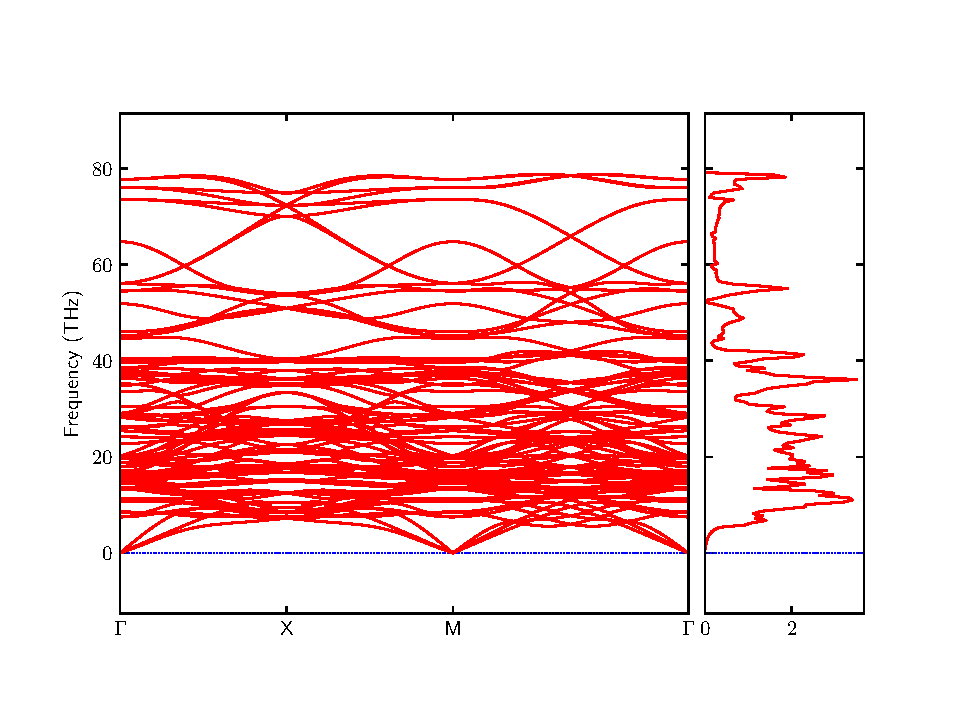
\includegraphics[width=\textwidth]{fig/simulation/band_dos_ltt.pdf}
    \caption[LTT Phonons (PBESol)]{Phonons in LTT phase with PBESol functional. Units are meV (the label is wrong).}
    \label{fig:ltt_ps}
\end{figure}

\begin{figure}
    \centering
    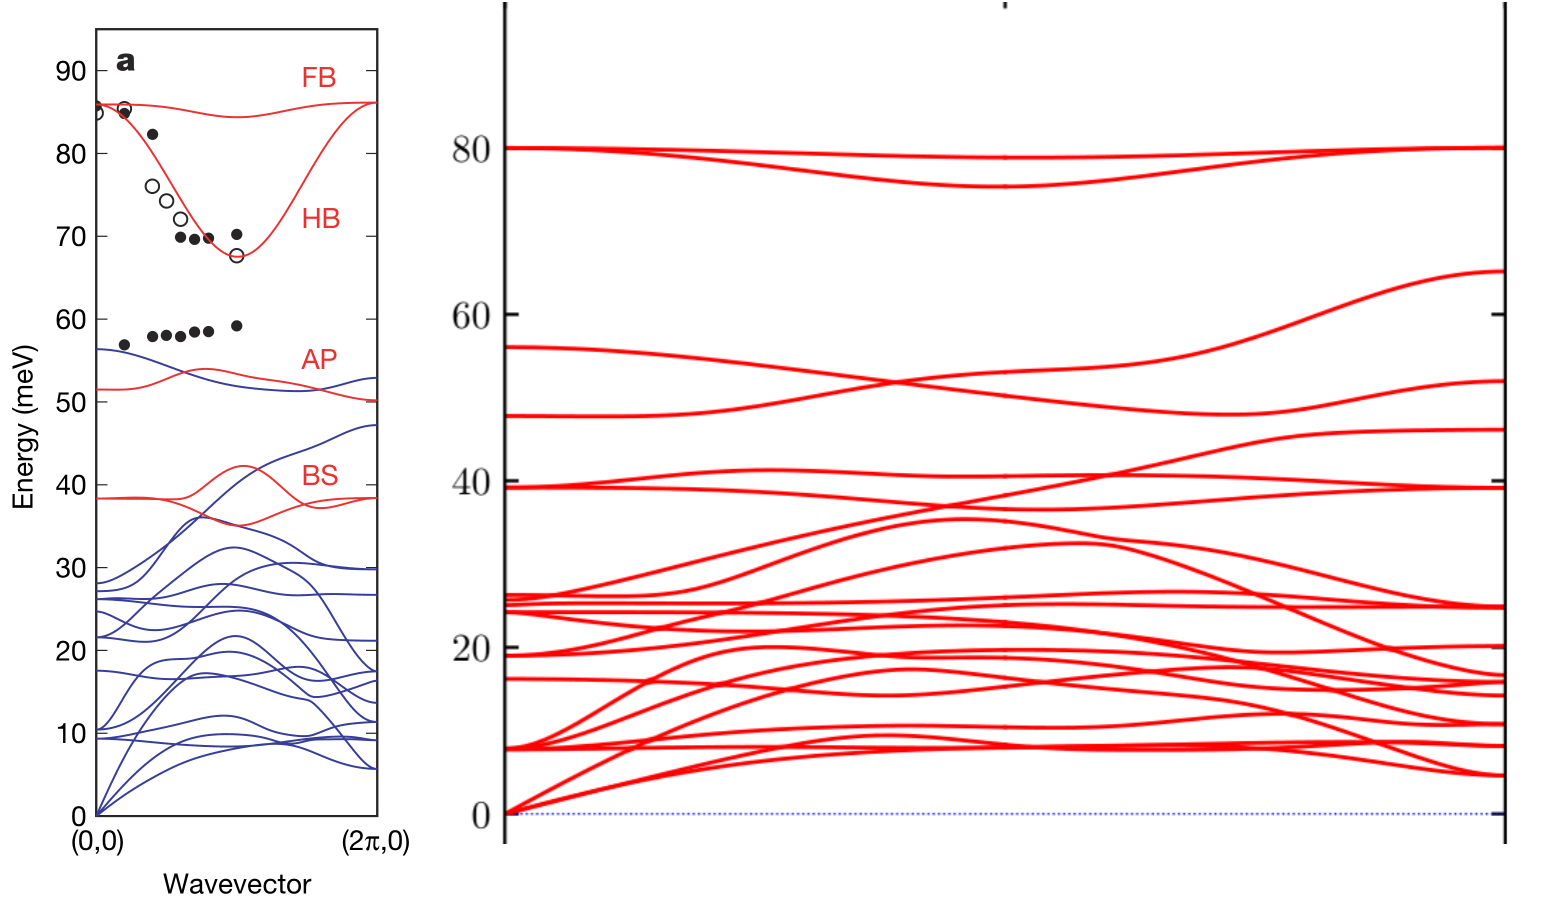
\includegraphics[width=\textwidth]{fig/simulation/giu_compare.png}
    \caption{Comparison of our AFM I4/mmm phonon dispersion with giustino et al. metallic phonons including e-ph coupling.}
    \label{fig:giu_compare}
\end{figure}



\begin{figure}
    \centering
    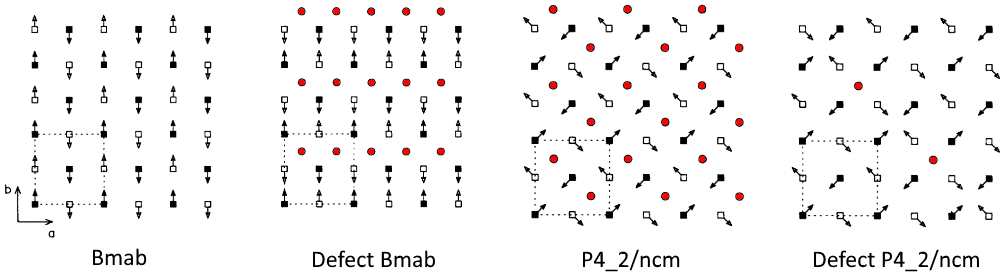
\includegraphics[width=\textwidth]{fig/simulation/oint.png}
    \caption[Illustration of interstitial positions]{Illustration of interstitial oxygen in-plane ($a$-$b$) location with respect to the apical oxygen displacements in the rock-salt layer. Open squares represent apical oxygens `hanging down' while closed squares represent apical oxygens `sticking up'. Interstitial oxygen are red circles. Adapted from \cite{Tranquada1995}.}
    \label{fig:oint_location}
\end{figure}

\begin{table}[b]
    \centering
    \begin{tabular}{@{}lllll@{}}
\toprule
Phase                   & Space Group & $\text{O}_\text{i}^x$ & $\text{O}_\text{i}^y$ & $\text{O}_\text{i}^z$ \\ \midrule
HTT                     & I4/mmm (139)      &         &         &         \\
HTT + O$_\text{i}$      & P-42m  (111)    & 0.125   & 0.125   & 0.25    \\
HTT + O$_\text{i}$      & Cmm2 (35)       & 0.125   & 0.125   & 0.24    \\
LTO                     & Bmab (64)       &         &         &         \\
LTO + O$_\text{i}$      & P2 (3)    & 0.125   & 0.125   & 0.25    \\
LTO + O$_\text{i}$      & P2 (3)         & 0.125   & 0.125   & 0.24    \\
LTO$_\text{defect}$     & Pmna (53)       &         &         &         \\
LTO$_\text{defect}$ + O$_\text{i}$ & P2 (3)         & 0.875   & 0.375   & 0.25    \\
LTO$_\text{defect}$ + O$_\text{i}$ & P2 (3)         & 0.875   & 0.375   & 0.24    \\
LTT                     & P4$_2$/ncm (138)  &         &         &         \\
LTT + O$_\text{i}$      & P-4 (81)        & 0.375   & 0.125   & 0.25    \\
LTT + O$_\text{i}$      & P2 (3)         & 0.375   & 0.125   & 0.24    \\
LTT$_\text{defect}$               & Pmma (51)       &         &         &         \\
LTT$_\text{defect}$ + O$_\text{i}$ & Cmm2 (35)       & 0.875   & 0.375   & 0.25    \\
LTT$_\text{defect}$ + O$_\text{i}$ & Cmm2 (35)       & 0.875   & 0.375   & 0.24    \\ \bottomrule
\end{tabular}

    \caption[Oxygen interstitial phases]{Space group symmetry due to the introduction of an interstitial oxygen in various structures all described in a $2 \times 2 \times 1$ supercell of the Bmab (conventional) coordinate system. HTT, LTO and LTT are the usual phases as described in litterature \cite{Hucker2012}. The structures labeled defect is (A) in the LTO case: A stacking fault where the middle layer has its tilts reversed and (B) in the LTT case: A line along [110] with reversed tilts. Both are described in \cite{Tranquada1994} and are designed in order to `make room' for the interstitial oxygen (see Figure \ref{fig:oint_location}).}
    \label{tab:oint_locations}
\end{table}

\begin{table}[b]
    \centering
    \begin{tabular}{@{}lll@{}}
    \toprule
     & $E_0$ [eV] & $E_1$ [eV]            \\ \midrule
    HTT                     & -827.27669             & -829.76250 \\
    LTO                     & -828.29890             & -830.39658 \\
    LTO\_sfault              & -823.09516             & -830.03588 \\
    LTT                     & -828.04663             & -830.08248 \\
    LTT\_defect              & -826.03173             & -829.94243 \\ \bottomrule
    \end{tabular}
    \caption[Oxygen interstital phases: Energy]{Oxygen interstital phases: Energy. $E_0$ corresponds to the energy after inserting the interstitial oxygen, but before geometry optimization. $E_1$ is the total energy after optimization. Geomtry optimization performed on ionic positions only. Conclusion: It costs more energy to create the defect structure than you gain by making room for the interstitial.}
    \label{tab:oint_en}
\end{table}

